
\documentclass[twocolumn,twoside,showpacs,preprintnumbers,superscriptaddress,amsmath,amssymb,prc]{revtex4}

 \usepackage{cases}
 \usepackage{CJK}
 %\usepackage{ccmap}
 \usepackage{txfonts}
 \usepackage{mathrsfs}
 \usepackage{amssymb}
 \usepackage{graphicx}% Include figure files
 \usepackage{dcolumn}% Align table columns on decimal point
 \usepackage{bm}% bold math
 \usepackage{subfigure}
 \usepackage{floatflt}
 \usepackage{float}
 \usepackage{siunitx}
 \usepackage{rotating}
 \usepackage{tikz}
 \usepackage{physics}
 \usepackage{multirow}
 \usepackage[bookmarksnumbered,bookmarksopen,colorlinks,citecolor=blue,linkcolor=blue]{hyperref} %
 %\usepackage{booktabs}
 \usepackage{epsfig,graphics,psfrag,amsmath}
 \usepackage{sidecap}
 \usepackage{graphicx}% Include figure files
 %\bibliographystyle{apssamp}
 \bibliographystyle{apsrev}

\begin{document}


The isovector reorientation effect effectively eliminates the influence of the isoscalar potential, allowing for the extraction of isoscalar information with high sensitivity. In the peripheral scattering of a polarized deuteron beam on a heavy target, the isovector force, being attractive to proton and repulsive to neutron, acts like a torque on the deuteron
and causes an additional rotation. As a result, the following breakup carries the effect of the rotation,
which is sensitive to the isovector force.  Detailed simulations demonstrate that the angular
distribution of the correlated neutron and proton from the deuteron breakup is very sensitive to the
isovector potential, but insensitive to the isoscalar nuclear potential. The experimental observable is quite simple to achieve: one can measure the angular distribution of the relative momentum vector
of the neutron and the proton. It serves as a probe that is particularly sensitive to the symmetry energy in the region of unsaturated nuclear density. By utilizing this probe, the uncertainty in the density dependence of the symmetry energy can be effectively constrained. 
  
  
   \begin{figure}
    \centering
    
\includegraphics[width=0.4\textwidth]{zby_img/isovector_reorientaton.png}
\end{figure}
  


 In order to verify the feasibility of our experiment, Geant4 simulations
were conducted. ImQMD transport model was used as an event generator.
The density dependence of $E_{\mathrm{sym}}\left(\rho\right)$ effect
can be mimic by varying the parameter $\gamma$ in
\[
E_{\mathrm{sym}}\left(\rho\right)=\frac{C_{\mathrm{s,k}}}{2}\left(\frac{\rho}{\rho_{0}}\right)^{\frac{2}{3}}+\frac{C_{\mathrm{s,p}}}{2}\left(\frac{\rho}{\rho_{0}}\right)^{\gamma}
\]
where $C_{\mathrm{s,k}}$ and $C_{\mathrm{s,p}}$ are the symmetry
kinetic and potential energy parameters, respectively. The parameters
$\gamma$ varies from 0.5 to 0.8 to cover the current range of the
world data. In each $\gamma$ case, $10\,\mathrm{M}$ incident deuterons
are simulated. For an event marked as “detected”, we require that
the breakup protons are detected by PDCs and the neutrons generate
a total light output $Q>10\,\mathrm{MeVee}$ (electron equivalent)
in NEBULA.
 
 The reaction plane is
determined by the $\vec{p}^{\mathrm{n}}+\vec{p}^{\mathrm{p}}$. The
reference frame is built so that $z$ is on beam direction and $y$
is vertical. In order to see the reorientation effect of polarized
deuteron scattering, as an example, Fig. \ref{fig:4} present the
momentum of the protons and neutrons from the deuteron breakup at
different impact parameter b and g conditions for $190\,\mathrm{MeV/u}\:\vec{\mathrm{d}}+\prescript{124}{}{\mathrm{Sn}}$
with transverse polarization $P_{yy}=100\%$. It is shown that the
distribution of the transverse momentum difference $p_{x}^{\mathrm{p}}-p_{x}^{\mathrm{n}}$
exhibits obvious asymmetry along 0, while the sum of the transverse
momentum $p_{x}^{\mathrm{p}}+p_{x}^{\mathrm{n}}$ depends on $b$.
i.e., the larger b is, less momentum loss on $x$ direction is obtained.
Similar effects with $P_{zz}=100\%$ can be observed. 

\begin{figure}[h]
\noindent \begin{centering}
% 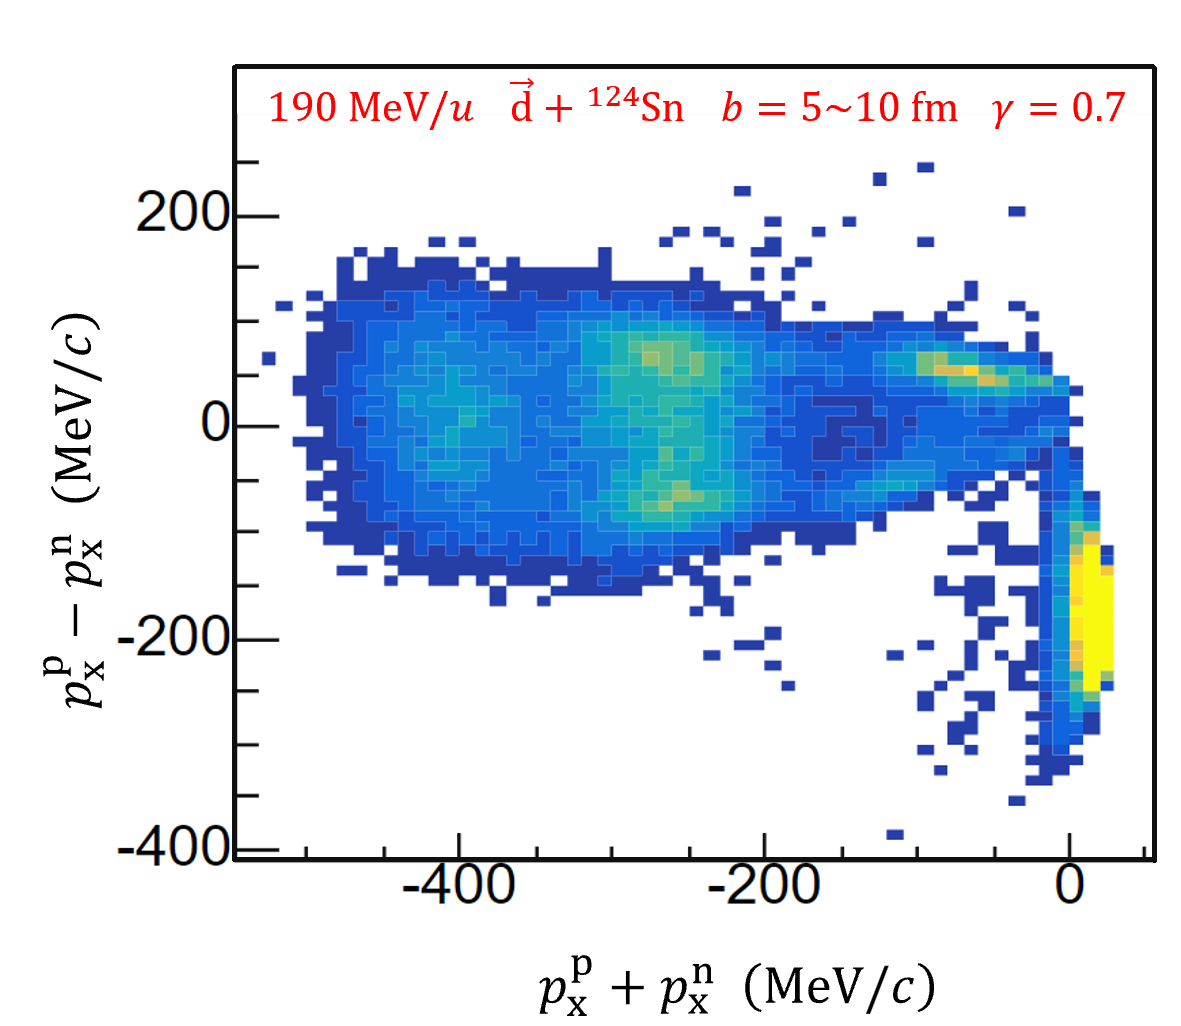
\includegraphics[width=8cm]{zby_img/4.png}
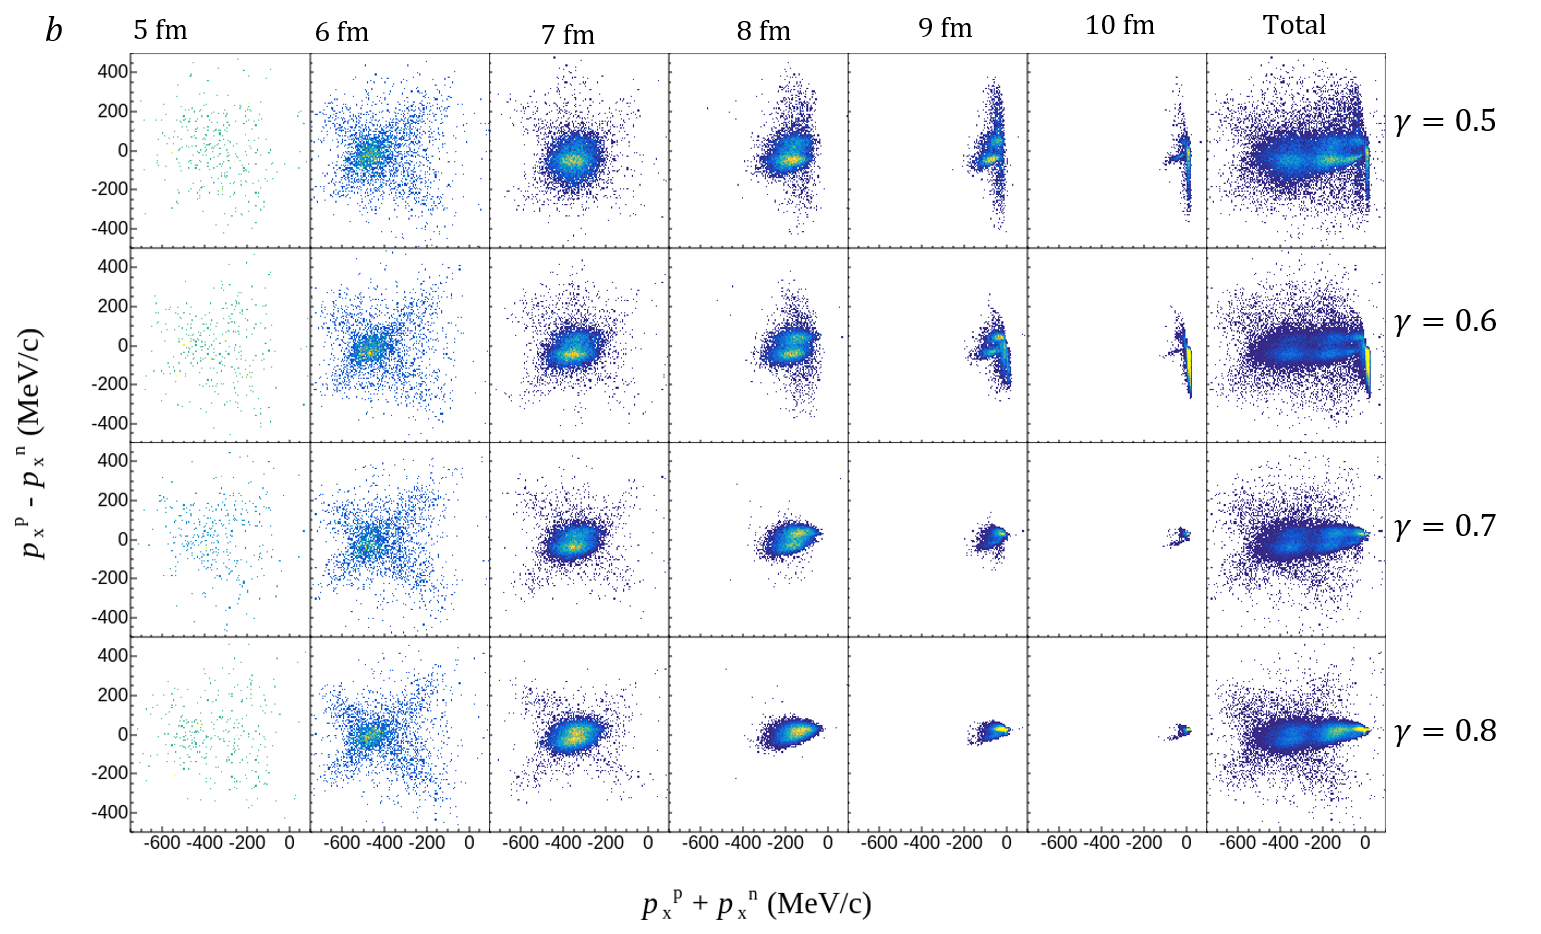
\includegraphics[width=8cm]{zby_img/distributionpzz1.png}
\par\end{centering}
\caption{\label{fig:4}Histogram for $p_{x}^{\mathrm{p}}-p_{x}^{\mathrm{n}}$
vs $p_{x}^{\mathrm{p}}+p_{x}^{\mathrm{n}}$with a beam polarization
$P_{zz}=100\%$.}
\end{figure}


Fig. \ref{fig:5} summarizes the distribution for $190\,\mathrm{MeV/u}\:\vec{\mathrm{d}}+\prescript{124}{}{\mathrm{Sn}}$
with $\gamma=0.6$. Here we show the results of longitudinal polarization
of the beam. A cut (Cut1) on the longitudinal momentum with $p_{z}^{\mathrm{p}}+p_{z}^{\mathrm{n}}>1150\,\mathrm{MeV/c}$
and $|p_{z}^{\mathrm{p}}-p_{z}^{\mathrm{n}}|<100\,\mathrm{MeV/c}$
is used to select the elastic breakup events. Further, the peripheral
events are selected by a second cut (Cut2) with $p_{x}^{\mathrm{p}}+p_{x}^{\mathrm{n}}>-200\,\mathrm{MeV/c}$
and $|p_{x}^{\mathrm{p}}-p_{x}^{\mathrm{n}}|<100\,\mathrm{MeV/c}$
on the transverse momentum. It can be observed that the distribution
of $p_{x}^{\mathrm{p}}-p_{x}^{\mathrm{n}}$ is asymmetric due to the
isovector reorientation effect.

\begin{figure}[h]
\noindent \begin{centering}
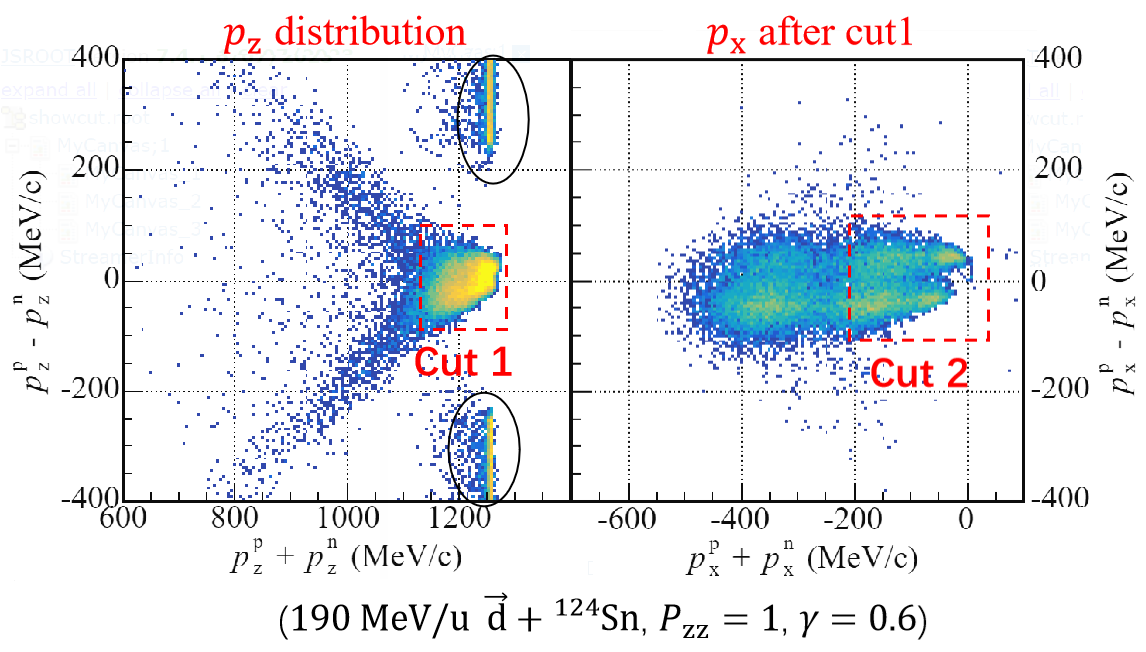
\includegraphics[width=8cm]{zby_img/5.png}
\par\end{centering}
\caption{\label{fig:5}The scattering plots of the momenta of the protons and
neutrons from deuteron breakup. Left: $p_{z}^{\mathrm{p}}-p_{z}^{\mathrm{n}}$
vs $p_{z}^{\mathrm{p}}+p_{z}^{\mathrm{n}}$ , Right: $p_{x}^{\mathrm{p}}-p_{x}^{\mathrm{n}}$
vs $p_{x}^{\mathrm{p}}+p_{x}^{\mathrm{n}}$ with Cut1.}
\end{figure}

\begin{figure}[h]
\noindent \begin{centering}
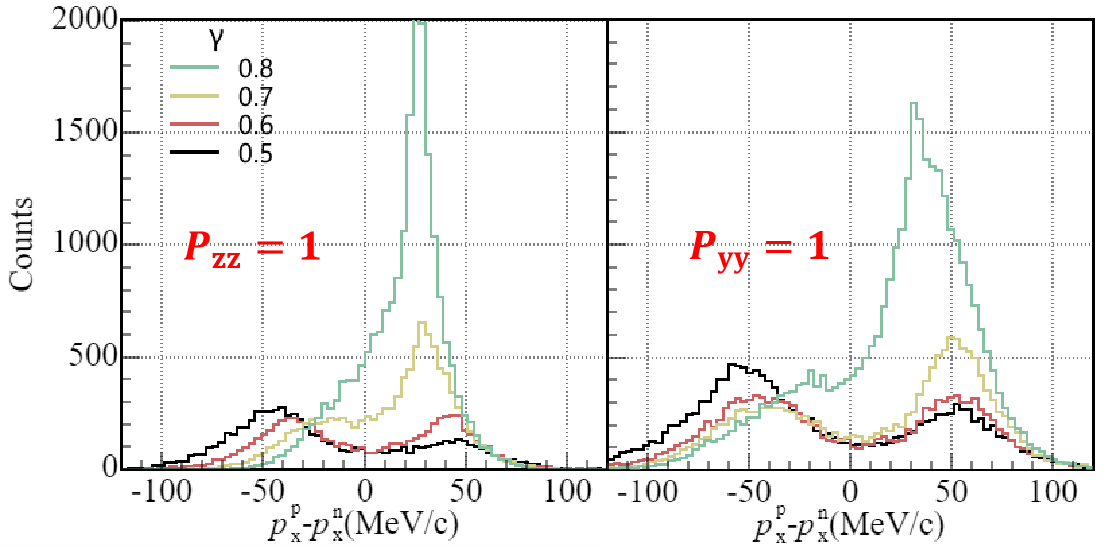
\includegraphics[width=8cm]{zby_img/6.png}
\par\end{centering}
\caption{\label{fig:6}$p_{x}^{\mathrm{p}}-p_{x}^{\mathrm{n}}$ distributions
for longitudinally and vertically polarized $190\,\mathrm{MeV/u}$
deuteron beam scattering on $\prescript{124}{}{\mathrm{Sn}}$ with
different $\gamma$ parameters.}
\end{figure}

In order to quantify the effect by varying the $E_{\mathrm{sym}}\left(\rho\right)$,
Fig. \ref{fig:6} presents the projected distribution of $p_{x}^{\mathrm{p}}-p_{x}^{\mathrm{n}}$
at different $\gamma$ values where cuts 1 and 2 are imposed. It is
shown that, for both polarization cases $P_{zz}$ and $P_{yy}$ ,
the asymmetric feature of $p_{x}^{\mathrm{p}}-p_{x}^{\mathrm{n}}$
around zero is evident. The component of $p_{x}^{\mathrm{p}}-p_{x}^{\mathrm{n}}>0$
is more abundant with increasing the stiffness of $E_{\mathrm{sym}}\left(\rho\right)$.
While in the unpolarized beam case, the distribution becomes symmetric,
regardless of the variation of $\gamma$.

We further define the yield ratio $R=\frac{Y\left(p_{x}^{\mathrm{p}}-p_{x}^{\mathrm{n}}>0\right)}{Y\left(p_{x}^{\mathrm{p}}-p_{x}^{\mathrm{n}}<0\right)}$.
Fig. \ref{fig:7} presents the distribution of $R$ as a function
of $\gamma$ for three reactions $\vec{\mathrm{d}}+\prescript{112}{}{\mathrm{Sn}}$,
$\vec{\mathrm{d}}+\prescript{124}{}{\mathrm{Sn}}$ and $\vec{\mathrm{d}}+\prescript{208}{}{\mathrm{Pb}}$.
It is shown that $R$ is very sensitive on the variation of $\gamma$,
giving $R$ as a robust observable of the isovector reorientation
effect and a clean probe to constraint the stiffness of $E_{\mathrm{sym}}\left(\rho\right)$. 

\begin{figure}[H]
\noindent \begin{centering}
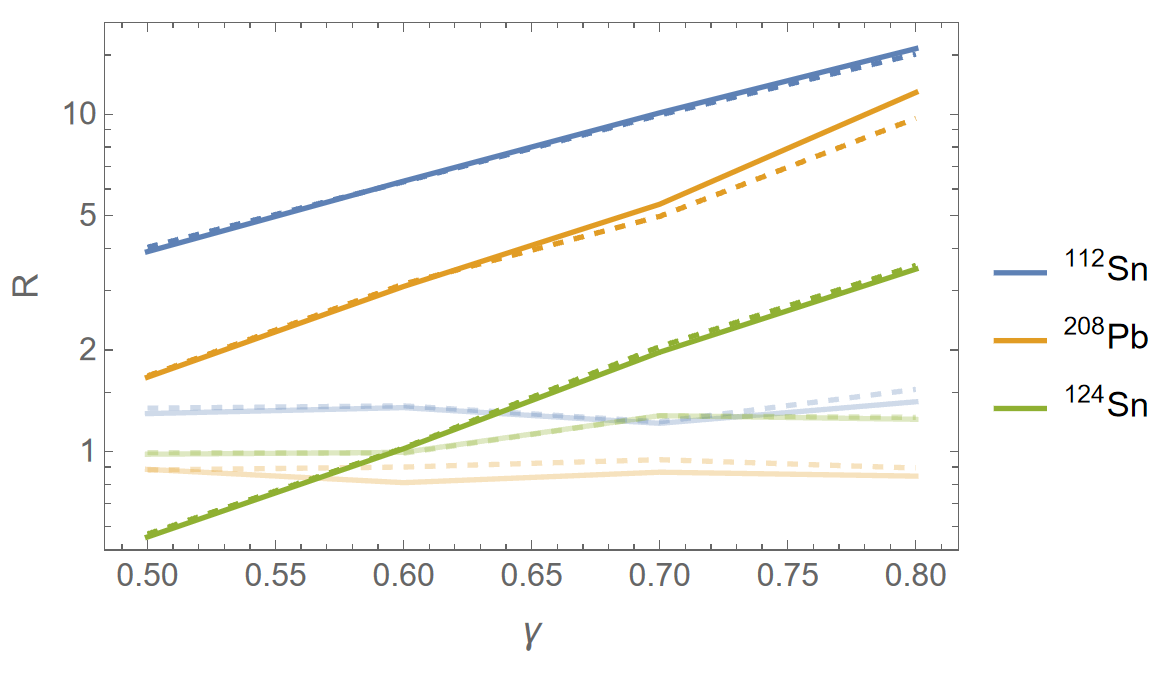
\includegraphics[width=9cm]{zby_img/7.png}
\par\end{centering}
\caption{\label{fig:7} The observable R (yield ratio of $p_{x}^{\mathrm{p}}-p_{x}^{\mathrm{n}}>0$
over $p_{x}^{\mathrm{p}}-p_{x}^{\mathrm{n}}<0$) as a function of
$\gamma$ for the longitudinally polarized ($P_{zz}=1$, in bright
colors) and unpolarized ($P_{zz}=0$, in shadow colors) deuterons
scattering on $\prescript{112}{}{\mathrm{Sn}}$, $\prescript{124}{}{\mathrm{Sn}}$
and $\prescript{208}{}{\mathrm{Pb}}$ targets. Those solid (dashed)
lines represent the simulation results without (with) the detector
uncertainties. The beam energy here is still $190\,\mathrm{MeV/u}$. }
\end{figure}




Using the ImQMD model and Geant4 simulation tools, deuteron-induced
reactions on heavy target nuclei with $190\,\mathrm{MeV/u}$ incident
energies have been studied. It is found that, due to the isovector
potential, there is a significant difference between the elastic scattering
angles of protons and neutrons in peripheral reactions. The distribution
of the transverse momentum difference $p_{x}^{\mathrm{p}}-p_{x}^{\mathrm{n}}$
varies a lot among different symmetry energy models. More specifically,
the yield ratio $R$ representing this distribution is very sensitive
to the model parameter $\gamma$. Therefore, a new probe is promoted
to be a promising candidate to constrain the symmetry energy at sub-saturation
densities. It is noteworthy that this probe is only effective for
longitudinally polarized beam, indicating the significance for polarization-related
techniques in our proposed experiment. 
\end{document}